% multiple1902 <multiple1902@gmail.com>
% intro.tex
% Copyright 2011~2012, multiple1902 (Weisi Dai)
% https://code.google.com/p/xjtuthesis/
% 
% It is strongly recommended that you read documentations located at
%   http://code.google.com/p/xjtuthesis/wiki/Landing?tm=6
% in advance of your compilation if you have not read them before.
%
% This work may be distributed and/or modified under the
% conditions of the LaTeX Project Public License, either version 1.3
% of this license or (at your option) any later version.
% The latest version of this license is in
%   http://www.latex-project.org/lppl.txt
% and version 1.3 or later is part of all distributions of LaTeX
% version 2005/12/01 or later.
%
% This work has the LPPL maintenance status `maintained'.
% 
% The Current Maintainer of this work is Weisi Dai.
%

\chapter{系统分析、评估及优化}
\echapter{Evaluation}
\label{EvaluationChapter}
\section{系统数据及分析}
\setcounter{subsubsection}{0}
\par
本部分首先给出方案的测试结果,然后根据测试结果对系统做出理论分析和评估。
\par
由于命名数据网测试环境硬件规模的限制,当前的测试并不是大规模的。在少数的几个节点运行多个游戏应用,且它们都处在一个小立方体,处在对方的感知范围内的情况下,本文重点度量了每个节点的出入总流量和,即平均吞吐量(单位:字节/秒),由各个节点运行Wireshark进行抓包,对每个相关的TCP包的负载字段的长度求平均得到;平均位置更新频率(单位:次/秒),由每个游戏应用分别计时、记录;平均每次获得更新对应的延迟时间(单位:毫秒),由每个游戏应用在利用操作系统提供的时间进行时间同步后分别记录;以及发现时间,即所有节点完成其他节点的发现、渲染所用时间最长的节点用的时间(单位:毫秒),由每个游戏应用分别计时。
\par
在上述条件和测试方案下,我们得到了表\ref{tab:preliminaryResults}的测试结果,并以此对本文描述的初步设计方案做以量化和归纳。表\ref{tab:preliminaryResults}的测试结果来自于时长为3分钟的应用运行;应用数量从2到8,基本可以体现实际环境下每个立方体中对象的数量。
\begin{table}[h!]
          \centering
          \caption{实现方案测试结果表}
          \label{tab:preliminaryResults}
          \wuhao
          \begin{tabular}{cccccc} \toprule 
          	节点数 & 应用数 & 平均吞吐量(Byte/s) & 平均更新频率(次/s) & 平均延迟(ms) & 发现时间(ms) \\ \midrule
           	2 &    2 &    424 &    3.44 &   305.1 &   1002.4 \\ 
		2 &    4 &    538 &    3.28 &   312.5 &   1129.3 \\
          	3 &    3 &    611 &    3.22 &   313.8 &   1187.7 \\ 
           	3 &    6 &    782 &    3.04 &   356.2 &   1622.9 \\
		4 &	 4 &	   798 &    2.95 &   377.0 &   1454.1 \\
		4 &	 8 &	   936 &    2.89 &   392.2 &   1636.6 \\
\bottomrule
          \end{tabular}
\end{table}
\par
以第四行为例解释表的内容。该行体现了,在三台计算机上同时运行六个游戏实体,每台计算机运行两个时,平均位置更新的频率为1秒钟3.04次;运行游戏的3各节点的平均吞吐量为782B/s;平均更新频率为356.2秒一次;发现过程经历时间最长的节点用了1.6秒才完成了对整个环境的准确构建。
\par
表中的数据有几点值得注意:首先,1秒3次左右的计划更新频率是常数配置时设定的,其频率略低,主要原因是当前NDN路由进程位置应答的新鲜时间最少为1秒,因而应用需要使用版本信息对位置进行过滤,过滤选择字段会带来名称长度的大大加长,因而还需要通过更多地测试对该值做出优化。其次,平均吞吐量字段随节点数及游戏实体数的增长是增量线性的,造成的主要原因是同步模块步骤一,即发现部分,带来的吞吐量是固定的;而更新部分,即步骤二,带来的吞吐量是线性增长的。再次,第四行测试数据在时间上相对偏差较大,推测的主要原因是其它应用导致的当时路由节点的瞬时流量较大。最后,测试数据可能会丧失一定的代表性,主要由于一半的数据来自于同一个物理节点运行多个游戏应用,这是在实际应用场合中不应该出现的。
\par
考虑到当前的命名数据网协议仍然是TCP的负载,由底层的TCP/IP协议本身会带来一定的头部,本文在度量吞吐量时只计算了TCP协议负载的字节数。出于同样原因,本文认为在NDN完成完全摒弃TCP/IP的部署后,本设计方案能在效能上获得提升。
\par
为了反映表中数据变化的趋势,下面数个折线图体现了表中字段随节点个数的变化。图\ref{fig:Throughput}体现了平均吞吐量是增量线性的。其基础值取决于发现模块,即同步第一步的数据请求的大小。
\begin{figure}[!h]
	\centering
	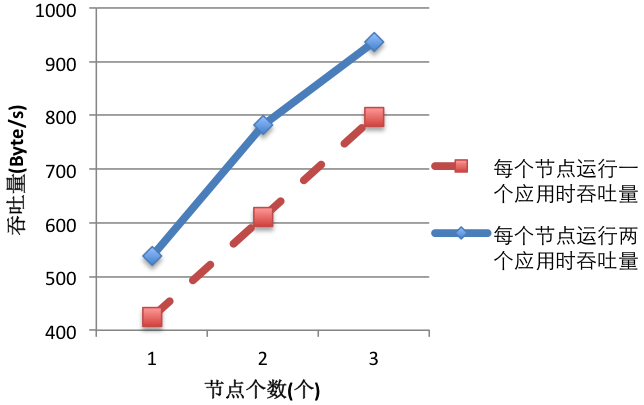
\includegraphics[width=6.67cm]{ThroughputFig.png}
	\caption{每个节点运行一个、两个应用时的平均吞吐量}
	\label{fig:Throughput}
\end{figure}
\par
图\ref{fig:Frequency}体现了更新频率的变化。可以看出随着节点数增多,更新频率呈下降趋势,但是仍在设定的3个左右。
\begin{figure}[!h]
	\centering
	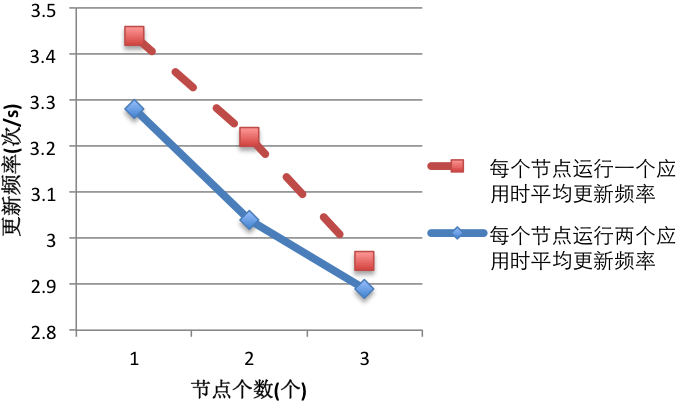
\includegraphics[width=6.67cm]{Frequency.png}
	\caption{每个节点运行一个、两个应用时的更新频率}
	\label{fig:Frequency}
\end{figure}
\par
图\ref{fig:DelayTime}体现了延迟时间的变化。由于每一时刻的延迟时间极大的受到整个网络通路中各个节点的拥塞情况,和NDN进程的运行状态的影响,只有其平均值可以较好的反应该量变化的规律。定性的看,延迟时间是随节点数量增多而变大的,实际测试中体现了这一趋势。
\begin{figure}[!h]
	\centering
	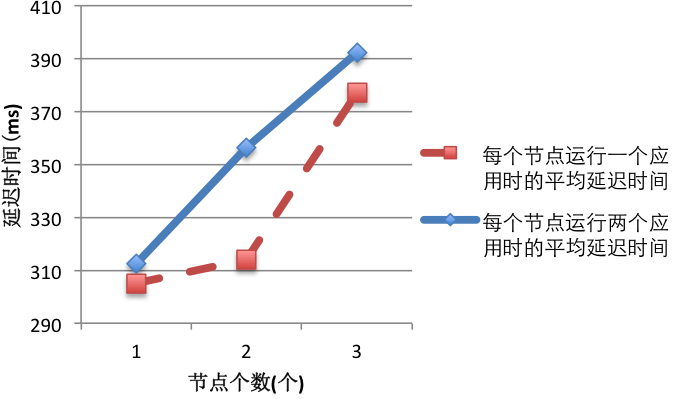
\includegraphics[width=6.67cm]{DelayTime.png}
	\caption{每个节点运行一个、两个应用时的延迟时间}
	\label{fig:DelayTime}
\end{figure}
\par
图\ref{fig:DiscoveryTime}体现了最长更新时间的变化。该量的测量容易存在疑义。因为每个节点加入该立方体的时间是较难完全同步的,所以随着新对象加入同一立方体加入,该立方体的状态,及状态变化的历史会变得更加复杂,使得之后加入的节点完成同步所用的时间增长。在此图中,发现所用时间最长的节点一律是最后一个加入的节点。该量测量的意义在于可以了解,在最坏情况下,新节点实现复杂区域的同步所用的时间是多少。
\begin{figure}[!h]
	\centering
	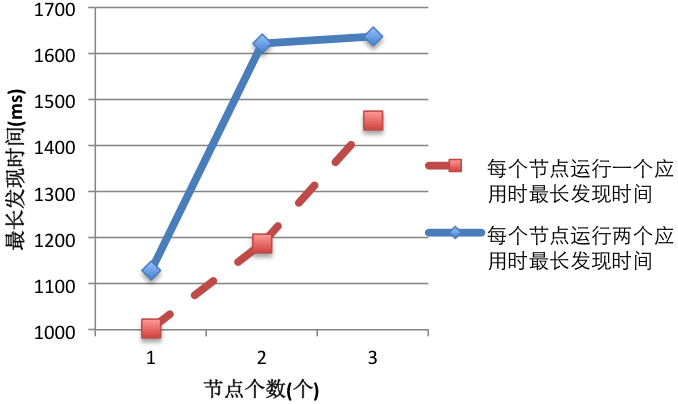
\includegraphics[width=6.67cm]{DiscoveryTime.png}
	\caption{每个节点运行一个、两个应用时的发现用最长时间}
	\label{fig:DiscoveryTime}
\end{figure}
\par
对应表\ref{tab:preliminaryResults}的测试结果,综合考虑在摒弃TCP/IP协议栈后会带来的效能提升,本文认为设计方案达到了需求分析部分提出的几点要求。在此对于上面提出的每一点重新做以分析和总结。
\subsubsection{局部性}
八叉树划分,并且只对自己感兴趣的立方体进行同步体现了局部性的要求。如此发出数据请求和注册名称前缀会使得发出数据请求的节点不发出多余的信息,而接收到数据请求的节点收到的内容逻辑上也都和自己相关。
\subsubsection{实时性}
本文的设计方案从两方面满足实时性的要求。一方面由于命名空间是共享的,通过合理的八叉树大小的配置,广播发现数据请求可能被多个节点共享的可能性较大。另一方面,每个数据请求只获取新鲜数据,并且每个数据应答有相应的新鲜周期,所以更新过程不会受到过期数据的影响。
\subsubsection{大规模可拓展性}
通过将状态同步和数据同步分离,将广播发现过程和位置、动作更新过程分离,本文的设计方案在理论上有较高的效率。而下面所述的系统优化将有助于可拓展性进一步提升。
\subsubsection{健壮性}
这里分别讨论网络分块、发现数据请求乱序、丢包和位置数据请求乱序、丢包造成的影响。由于发现数据请求一直在被定时广播,出现网络分区后,一旦连通性恢复,节点间的互相发现不应该受到影响。同时,发现数据请求的应答出现丢包或是乱序对系统没有严重影响。对于丢包的情况,请求发送方会收到请求超时并重新发送发现请求;对于乱序的情况,位置应答而不是发现应答对渲染哪些对象有决定权,所以也不会对系统有影响。位置数据请求如果丢包,会导致请求方短时无法更新对象的位置;而位置数据请求会包含本地时间的时间戳,如果出现乱序,时间戳靠后的位置被渲染后收到时间戳考前的位置,后者不会被渲染。
\par
综上,系统对达到了理论分析中提出的要求;并对网络可能出现的异常有一定抵抗力。
\section{系统优化}
\label{OptimizationSection}
\par
本部分记述已经实际应用于项目实现中的优化。
\subsection{多个数据请求合一}
\label{MultiLevelOptimizationSection}
\par
考虑到设计方案在用立方体块表示球形的感知范围,为了使表示准确,要使用的立方体块数较多。如果对于每个立方体分别发出数据请求,数据请求的数量会较多。
\par
利用八叉树划分虚拟环境的优势之一是利用八叉树的层次结构,即不止对叶子节点发出发现数据请求。在数据请求的发出方了解到自己的数据请求可以利用八叉树结构进行合并时,数据请求的发出方会对最后的哈希字段做以重新的编码。对于上述用例,需要发出的数据请求发生了如下变化。首先,名称不一定总是指向最底层的立方体块;其次,Digest的编码要表示本Digest是否为整个叶立方体的块的;如果不是 ,是叶立方体的哪个子块的。
\par
如此优化带来的好处有大大减少发出的数据请求数量,和注册的前缀数量。原本的思路中,每个大小立方体对应一个独立数据请求和注册前缀。现在,注册的前缀只用包括几个包含感知范围的立方体的特定层的父节点;而发出的数据请求的数量会动态的发生变化,其变化与之后的渐进性发现的优化思路有关。另外,这样的优化更加自然,因为其利用了八叉树本身提供的树形结构,而不是将其等同于一维编码,例如基于康拓配对或希尔伯特曲线的划分。
\par
\subsection{渐进性发现}
\par
渐进性发现的含义有两点。允许收到数据请求的节点在不具有完整的被请求信息时进行回复;以及允许每个节点动态的调整自己的感知范围大小。
\par
第一点的问题来自于上一则优化。
\par
由于数据请求的合一,节点收到的数据请求包含的区域不一定和本地拥有的或感兴趣的信息完全吻合,从而为节点做出应答带来了困难。
\par
当数据请求包含的区域是本地感兴趣的区域的子集时,节点可以通过解码、匹配到对应区域并作答;
\par
当数据请求包含的区域与本地感兴趣的区域完全不相交时,节点不予作答并在预设时间过去后请求超时;
\par
而考虑二者的中间情况,即当数据请求包含的区域与本地感兴趣的区域部分相交,换言之,本地感兴趣的区域包括数据请求包含区域的子集。节点如果作答,可能导致请求者收到不完整的答案,请求者需要根据不完整的答案重新核实,并修正自己的哈希值字段,然后重新发布发现数据请求,并且希望这次的哈希值同有着不完整信息的节点的哈希值相同,从而其不会作答。在此期间,有完整数据的节点可能也会收到数据请求 ,并试图作答,但是为了保证收发平衡,其答案会由于重复而被路由节点丢弃。最终导致的结果是数据请求节点为了获得完整的信息,反而付出了更长的时间。节点如果不作答,则对于接收节点而言,自己接收了没有意义的信息;对于发送节点而言,相当于其要求网络中的接收节点拥有的区域与自己发出的请求代表的区域完全吻合,这样的情况可能较少出现。对此,本文提出了一个折中方案。接收节点可以作答,但是其会主动延迟应答发出的时间。延迟时间和二者区域的重合程度成反比,即区域的交集占数据请求中区域的比例越大,延迟的时间越少。而最初叙述的两种简单情况也可以视为二者的比例为1时,接收请求的节点立刻作答;二者的比例为0时,接收节点推迟无穷大时间。
\par
在解决了这一问题后,渐进性发现还有一点含义,即允许节点根据当前所在虚拟环境的密集程度和网络是否拥塞动态的调整自己的感知范围。这一点即为kNN问题的实际用例。数据请求指向的立方体不再由固定的感知范围定义,而由节点根据自己了解到的周围对象数量的多少步进式的动态调整。
\par
例如,节点首先试图获取R范围内包含的立方体中的对象,如果对象数量未达到k个,则R自增一个单位,直到对象数量满足要求。对于收到的所有对象名称,节点根据其位置进行排序,并且只渲染其中最近的k个。这里R自增一个单位的方式可以利用kd树的kNN查找,由于在\ref{kNNIntroSection}部分已经有所介绍,这里不再赘述。另外一种自增的方式是实际考虑本地对象当前的速度和朝向,并且加入该朝向上的一个叶子立方体。后者的实现可能会不太稳定。
\subsection{事件驱动为主的请求发送}
\par
在上述的设计思路中,发现数据请求是定期广播的。为了保证发现的及时性,广播的周期不能很长,而为了减少流量,广播的周期也不能过短。本部分引入事件驱动为主的请求发送,从而进一步减少广播发布的数据请求数量。简而言之,每当本地对象新启动游戏,移动或渐进性发现导致了感知范围包含新的立方体时,节点对该立方体以较高的频率发布广播发现数据请求。其它情况下,节点对该立方体以较低的频率发布广播发现数据请求。这样做设计上较为自然,即在已知区域基本达到稳态后,各个节点基本不需要再通过广播发现数据请求维持状态上的同步从而了解对象的去留,而仅通过单播的对象位置信息,就可以清楚对象的去留。而当节点对新的立方体产生兴趣时,无论是因为节点加入、感知范围扩大还是本地对象移动,节点应当积极的获取新立方体中的状态并与其同步。在这一过程中并不可以完全摒弃低频率的广播数据请求发送。一方面在特定的网络连接下,广播数据请求可以促进新的节点加入且其名称被一个感兴趣的节点发现后,更早的被别的感兴趣的节点发现;另一方面,广播数据请求可以使得游戏从一些网络异常现象中恢复,比如网络分块。
\section{其它设计思路及对比}
\label{ComparisonSection}
\par
分析和评估的重点内容是和其它设计思路的对比。本部分记述设计过程中作者所主要考虑的其它设计思路,并和其一一做以对比。下面叙述的几个设计思路分为两大种类,第一种是基于NDN网络的,由作者在项目初期提出,经过理论分析后,作者认为无法很好的描述项目的需求;第二种是基于IP网络的,由别的研究人员在过去的10年中提出,与这些方案的对比较难进行,因为NDN网络还处于试验阶段,且我们缺乏的硬件条件和测试标准使得实际的测试有说服力。
\subsection{基于位置敏感哈希的划分}
\par
LSH方法的原理在背景部分已经有所介绍。基于LSH的方案不同于本文所提的方案,主要在于不再采用八叉树对虚拟空间进行划分,而采用两组预定的p稳定的哈希函数对虚拟空间进行划分。这里依然把LSH视为划分,是为了更直接的体现共享命名空间的概念。划分之后的步骤同本文重点描述的方案相近,但是可以更好的利用如\cite{LSHKNNRef}中描述的基于LSH的kNN算法。
\par
对于一个输入坐标(x, y, z),第一组k个哈希函数得到一个k维向量,对于该k维向量,第二组哈希函数得到一个值,即为该坐标所属于的虚拟分区桶编号。在第一步中使用多个函数的原因是用多组相交的平面可以更好的划分出虚拟空间对应的形状,并用其模拟球形的感知范围。采取这样的划分的原本目的亦是如此,即通过多个哈希函数的限制反映球形的感知范围,如图即为二维输入下圆形感知范围的模仿。
\par
然而在实际测试中,随机在本应用的虚拟环境中生成10000个点和哈希函数参数,利用2稳定的LSH寻找kNN得到的结果如表\ref{tab:LSHTable}所示。其中线性查找的点占的比例的含义是落在附近\footnote{在本例中,经过调节,哈希桶的范围被定义为100时综合效果较好}的哈希桶中,距离被用于确定是否在给定范围R\footnote{在本例512*512*512的虚拟环境中,R的值由欧几里得距离定义,具体取为40000}内的点,占全部10000个点的百分比。在该表中我们重点关注的量是kNN寻找的准确度,即在R范围内,LSH找到的点的个数占到实际应该出现的点的总数的百分比。就该字段而言,如表\ref{tab:LSHTable}所示,该算法的效果并不良好:为了使准确度达到近90\%,不仅要采用6个哈希函数,而且近一半的点被进行了线性查找。出现不良效果的问题在于步骤二。如果认为桶的数量足够多,不考虑取模对值的影响,在应用了第二组哈希函数后,整个过程的效果变为在第一步中仅运用一个哈希函数,即用两个平行的平面对三维虚拟空间进行划分。
\begin{table}[h!]
          \centering
          \caption{LSH方案的测试结果}
          \label{tab:LSHTable}
          \wuhao
          \begin{tabular}{ccccc} \toprule 
		哈希函数个数 & 哈希桶数量 & 线性查找的点占的比例(\%) & kNN查找的准确度(\%) \\ \midrule
          	3 &    $2^{14}$ &  6.7  &  34.7  \\ 
		3 &    $2^{20}$ &  5.9  &  33.6  \\
		4 &    $2^{14}$ &  13.8 & 43.1 \\ 
		4 &    $2^{20}$ &  12.9 & 42.4 \\
		5 &    $2^{14}$ &  26.4 & 65.1 \\
		5 &    $2^{20}$ &  26.2 & 65.1 \\
		6 &    $2^{14}$ &  49.7 & 89.6 \\
		6 &    $2^{20}$ &  48.4 & 88.4 \\
\bottomrule
          \end{tabular}
\end{table}
\par
除此之外,LSH本身并不适合三维,或是综合考虑时间后,四维,的用例。因为,第一组哈希函数的应用可以认为是在丢失一定量信息的高维到低维的维度缩减,而为了保证高维下的距离相对关系在维度缩减后仍有较高的概率保持不变,第一组函数往往需要选取多于4个。对于我们的用例,输入量本身的维度很低,维度减少并不是需要考虑的核心问题。
\par
综上所述,再加上LSH方法不能很好的应用多层的划分(如果直接采用值大小的多层划分,LSH依然存在边界问题,即不能很好的解决最初提出时希望解决的球形划分的问题),我们认为基于LSH划分的思路不会在表现上优于本文主要描述的方案。本文所用的LSH测试方案可以在作者的Github站点找到\footnote{作者的LSH相关的测试,https://github.com/zhehaowang/PStableLSHC,\newline以及https://github.com/zhehaowang/PStableLSHCSharp}。
\subsection{基于可逆转Bloom Filter的知识表达}
\label{IBFComparisonSection}
\par
可逆转的Bloom Filter(Invertible Bloom Filter, IBF)的原理在\ref{IBFIntroSection}部分已经有所介绍。基于IBF的设计方案的提出原本是为了用立方体的对象名称集的IBF取代哈希值的知识表达字段,即发现数据请求名称中的最后一个组成部分。基于IBF的设计方案的交互过程可以系统时序图,图\ref{fig:IBFSSD}概括。
\begin{figure}[!h]
	\centering
	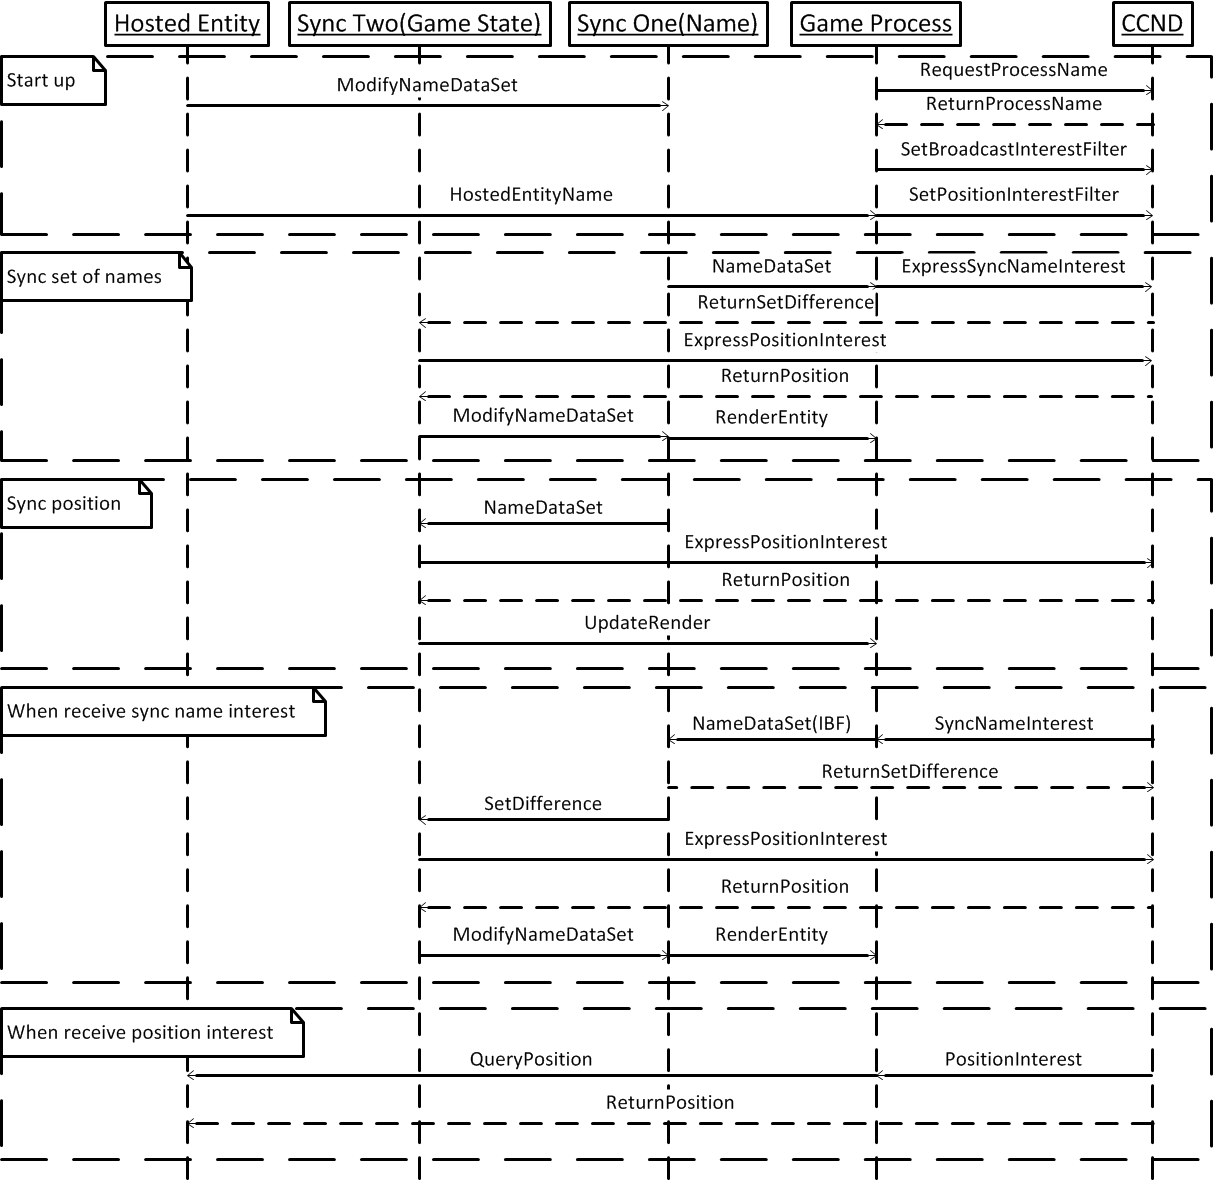
\includegraphics[width=0.9\textwidth]{ImplementationSSD.png}
	\caption{IBF方案的系统时序图}
	\label{fig:IBFSSD}
\end{figure}
\par
使用IBF的优势在于可以直接编码对象名称,在两个名称集的不同的元素数量较少的情况下,接收方有较高的概率可以直接解码出对象名称。因此,相对于文中重点描述的方案,基于IBF的方案在获取到数据请求的发送者拥有哪些名称上可以少一个数据应答的时间。另外,考虑到IBF的表现在两个名称集的交集较大,而差集很小的情况下较为出色,而名称集的同步从一个稳态过渡到另一个稳态的过程恰巧符合这个特点,IBF显得更加适合我们的用例。
\par
然而,IBF具有以下的缺点。首先,差集的恢复是概率性的,为了提高恢复的概率,IBF的大小必须提高,即拥有更多的哈希桶。这意味着广播数据请求的长度也会相应提高。由于广播数据请求会更多的被发送,其长度应该尽可能的被减小,而为了从10个名称中拥有90\%的概率恢复出3个不同的名称,IBF会为数据请求名称增加200个字节,这在作者认为是不值得的。其次,IBF无法很好的利用八叉树的层次结构。如果\ref{OptimizationSection}部分中头两点方案,除了广播发现数据请求的名称会变得过长外,在节点接收到的发现数据请求描述的区域和自己了解的区域不完全相同时,IBF会退化为普通BF,意味着其可能漏过不同的名称。
\par
为了更好的体现IBF存在的劣势,在此给出外部条件均为3个节点运行3个游戏实体的情况下,IBF和本文采用方案的测试结果的对比表。如表\ref{tab:IBFComparison}所示,由于发现所需的来回数减少了一个,IBF在发现所用最长时间上带来了较大的优势,但是吞吐量上带来的劣势过大。
\begin{table}[h!]
\centering
\begin{threeparttable}[h]
          \centering
          \caption{IBF方案测试结果对比表}
          \label{tab:IBFComparison}
          \wuhao
          \begin{tabular}{ccccc} \toprule 
		方案名 & 平均吞吐量(Byte/s) & 平均更新频率 (次/s) & 平均延迟 (ms) & 发现时间 (ms)\\ \midrule
          	IBF &    611 &    3.22 &   313.8 &   1187.7 \\ 
		Hash Digest\tnote{1} & 1472 & 3.16 & 314.8 & 877.8 \\ 
\bottomrule
          \end{tabular}
	\begin{tablenotes}
	\item[1] 即为本文方案。
	\end{tablenotes}
	\end{threeparttable}
\end{table}
\par
综上考虑,本文并没有最终使用基于IBF的设计方案。作者为测试用而实现的IBF结构可以在作者参与合作的Github站点找到\footnote{基于IBF和CCNx实现的游戏应用代码链接,https://github.com/CherryQu921/NDNMOG/tree/npc}。
\subsection{部分P2P思路}
\label{PartialP2PSection}
\par
部分P2P的思路的核心在于动态的选择某个节点,使其为某一个区域负责,即掌管该区域的名称集,并通知其它节点自己为该区域的负责人。由此,对该区域感兴趣的节点问网络的问题变成了谁是区域的负责人,而在拥有了负责人名称之后,节点的问题变为向负责人询问它的名称集,或是通知负责人自己的加入或是离开。如此,为了实现各个区域的同步,所有对该区域感兴趣的节点只用不断的请求负责节点的名称集即可。而在负责人离开后,其需要指定下一任负责人,或是通知各个感兴趣的节点进行选举,并将信息移交给下一任负责人。
\par
部分P2P是IP的P2P游戏联机的主要思路之一。其显著的优点在于除了负责人替换的策略外,控制相对简单,且完成同步所需的网络流量也可能会相对较小。
\par
本文并没有重点探究部分P2P的思路,一方面是因为负责人替换策略比上面描述的要复杂许多,因为要考虑负责人非正常离线等情况导致的信息无法正常交接,和负责人协商的过程本身也需要多个节点的同步和解决冲突。另一方面是因为我们的用例作为NDN多人联机游戏,数据存储的位置的重要性应该得到弱化,因此不希望采取一个依然拥有逻辑上的小规模“服务器”的策略。
\par
在这两种架构的选择背后有更深层的研究和讨论,目前并没有一种优于另一种的定量结论,二者的区别更多地是被看做设计理念上的不同。而本文描述的应用也可以看做是主观上希望尽可能的探究纯P2P结构的大型网络联机游戏的可能性。
\subsection{IP网络下的P2P实现}
\par
IP网络下有许多P2P多人联机游戏的实现方案。最为流行的思路是基于DHT中间层的。大体而言,是通过建立和维护一张将虚拟环境游戏状态映射到为该游戏状态负责的节点的IP地址或是到达该节点的下一跳IP地址的分布式哈希表,解决IP网络自组织多人联机游戏的核心问题:从哪里获取数据。在DHT的部署上或是哈希的内容上,不同文章的做法不尽相同。Pastry系统\cite{IPP2PMMORPG1}的思路是将参与游戏的所有节点和所有游戏对象的ID进行哈希;而\xjtuincite{IPP2PMMORPG2}先将虚拟环境进行划分,为每个分区动态的选择负责人,并将分区和负责人信息进行哈希,更加类似基于多播的Pub/Sub系统\cite{PubSubRef}。
\par
在这些思路中,DHT的存在体现了IP网络中“地址”扮演的重要性,同时也体现了,在拥有一个物理环境主持一个虚拟环境,二者不存在直接的映射;且就希望优化的量而言,传输效率是对物理环境的要求,而局部性是对虚拟环境的要求,的情况下,IP对物理环境或物理位置的过度强调,使得应用的设计并不自然。本文的NDN游戏应用将考虑的核心放在了“问网络怎样的问题”上,而不是“从哪里获取答案”上,更加贴近了应用层的开发理念,省去了不自然的DHT中间层,也利用了NDN网络对多播的天然支持,争取得到效率上最大化的提升。
\subsection{IP网络下的C/S实现}
\par
传统MMORPG是基于客户端/服务器结构实现的。服务器将为游戏状态及用户账户负责。C/S架构下的可拓展性是通过服务器集群实现的。多台服务器间可以通过局域网相连,比如Terazona\footnote{简单介绍,http://www.businesswire.com/news/home/20030303005397/en/Zona-Announces-Terazona-Network-Engine-Support-Capcom\#.U5pKKY0Ybb4}中描述的;或是组成计算网格,如Butterfly.net中\footnote{参考书籍,Official Butterfly.Net Game Developer's Guide}描述的。尽管这种架构通过增加服务器的数量,优化服务器的策略可以使得更多的玩家同时享受服务,它仍缺少自组织网络的灵活性,并且就目前的实施情况来看,服务器总是无法很好的应对服务需求的高峰期。同时,C/S架构的游戏限制了当今游戏的另一个发展趋势,用户开发游戏的部署。尽管像EverQuest等的游戏允许用户自主设计游戏扩展,然而安全和效率的问题仍然会限制这些拓展的数量和体积,因为他们都需要在为游戏状态负责的服务器上统一存在。
\par
尽管C/S架构存在许多潜在的问题,目前商业化的网络游戏仍然没有采用P2P架构的。目前P2P架构相对于C/S架构的优点更多只有于定性的理论分析。如\ref{PartialP2PSection}所述,二者是设计理念上的不同。而基于新网络架构的P2P实现可能会为两种架构的讨论带来新的思路,机遇和挑战。
\section{本章小结}
本章列举了经过实现和测试后得到的方案数据,并对数据做以了初步的分析。之后,本章对系统是否达到了需求中的要求进行了理论分析。在此之上,本章对系统提出了三点优化方案,目前三点方案已经实现,但是还没有进行系统的测试。最后,本章将本文的设计方案和我们早期的三种思路,和IP下的两种思路进行了对比。对于IBF和LSH的思路,本文给出了具体的测试数据;对于部分P2P的NDN思路和IP下的两种实现,由于环境相差较大或是设计理念不符,本文仅做出了理论分析。
